\chapter{開発準備}

\section{開発に利用したツールとその経緯}%例:レビュー内容
%必要ならここに大見出しの内容
%必要なら下のsubsectionを用いて小見出しをつかう
\subsection{Monaca}%:発表技法について
iOSとAndroidの両方のプラットフォームでアプリケーションを使いたいという陣川あさひ町会の要望を叶えるために、HTML5ハイブリッドアプリを開発することとした。iOSとAndroidには、「WebView」と呼ばれるブラウザの機能を持つコンポーネントが組み込まれている。HTML5ハイブリッドアプリとは、「WebView」にHTMLとCSS、JavaScriptを用いて開発するアプリケーションである。また、HTML5ハイブリッドアプリの開発ツールのなかからMonacaを選択した。MonacaはCordovaというオープンソースのフレームワークを(利用している)。また、MonacaにはMonacaクラウドIDE、Monaca Localkit、Monaca CLIの3種類の開発環境が存在する。MonacaクラウドIDEは、インターネットクラウド上で開発するため個人の開発環境に依存しない。Monaca Localkitは、MonacaクラウドIDEとは異なり、各メンバごとにローカルでの開発を可能とする。Monaca CLIは、MonacaクラウドIDEが提供するサービスを、コマンドライン形式で利用することを可能にする。

\begin{figure}[h]
  \begin{center}
  %\begin{flushleft}
    \begin{tabular}{c}

      % 1
      \begin{minipage}{0.7\hsize}
        \begin{center}
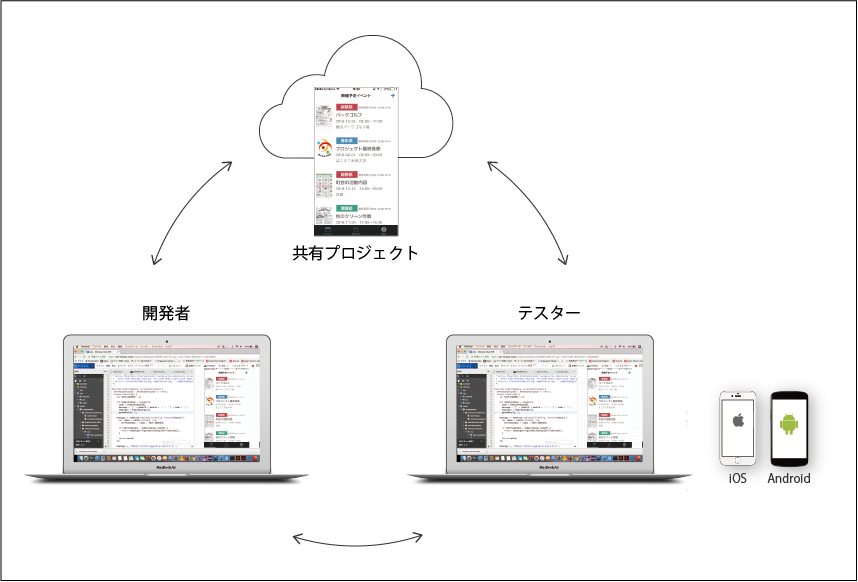
\includegraphics[width=10cm]{monaca_overview.eps}
          \hspace{1cm} %(a)観光スポットの紹介
        \end{center}
      \end{minipage}

    \end{tabular}
    \caption{Monacaでの開発イメージ}
    \label{fig:lena}
  \end{center}
  %\end{flushleft}
\end{figure}

\subsection{ニフティクラウド mobile backend}%:発表技法について
本アプリケーションの各情報を保存する場所として、mBaaSの1つであるニフティクラウド mobile backendを使用した。以下、NCMBとする。mBasSとは、サーバーの開発、運用を必要とせずユーザから直接見えない部分の機能をアプリに実装することを可能にするサービスである。NCMBは、プッシュ通知、会員管理と認証、SNS連携などの機能を提供しているサービスである。

\begin{figure}[htbp]
%\begin{flushleft}
  \begin{center}
    \begin{tabular}{c}

      % 1
      \begin{minipage}{0.7\hsize}
        \begin{center}
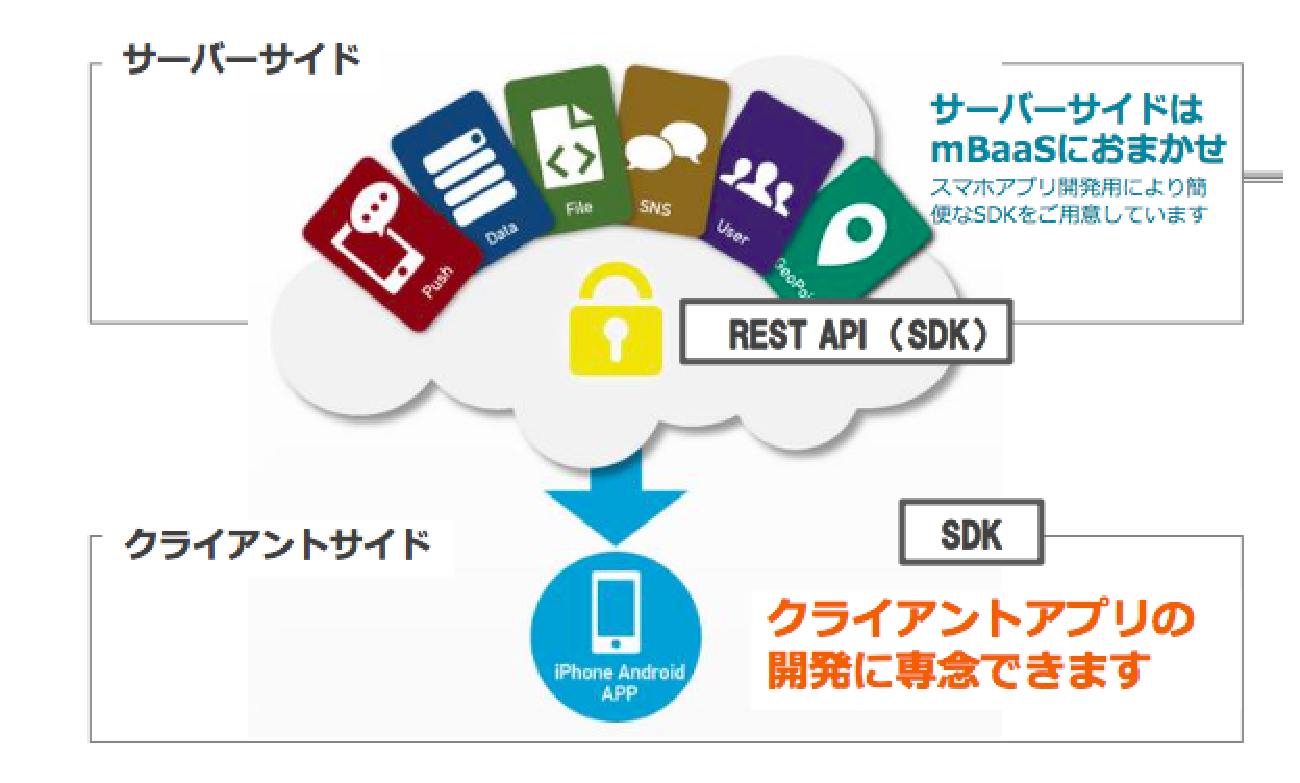
\includegraphics[width=10cm]{ncmb_overview.eps}
          \hspace{1cm} %(a)観光スポットの紹介
        \end{center}
      \end{minipage}

    \end{tabular}
    \caption{ニフティクラウド mobile backendのサービス内容}
    \label{fig:lena}
  \end{center}
  %\end{flushleft}
\end{figure}


\subsection{Git/Github}%:発表技法について
ソースコードのバージョン管理ツールとして、Git/GitHubを使用した。Gitはファイルの変更履歴をリポジトリと呼ばれる場所に保存する。そのため、一度編集したファイルを過去の状態に復元することや、編集箇所を表示することが可能となる。リポジトリの種類は、メンバのローカルPC内に存在するローカルリポジトリと、インターネット上に存在するリモートリポジトリの2種類である。リモートリポジトリでは、各メンバのファイルの変更履歴を保存し、共有する事が可能である。GitHubは、リモートリポジトリを提供するサービスの1つである。これにより、複数のメンバで同時に開発を進めることが可能となった。タスク管理には、Redmineというオープンソースソフトウェアを利用した。


\subsection{Redmine}%:発表技法について
Redmineでは、発生したタスクごとにチケットと呼ばれるものを発行する。その後、タスクの進捗に合わせて各チケットを新規、フィードバック、進行中(着手)、進行中、進行中(終了間際)、作業終了、レビュー中、完了、却下の9段階に分ける。また、チケットには担当者を指定し、チケットが更新される度に通知が来るようにウォッチャーと呼ばれるものに各メンバーを設定する。これにより、各メンバのタスクの進捗状況を把握することが可能となった。


\subsection{Illustrator}%:発表技法について
ポスター作成と開発するアプリケーションのイメージ図の作成にAdobe Illustratorを使用した。Adobe Illustratorはイラストやポスターなどデザインを描画するソフトウェアの1つである。

\section{環境構築}%例:レビュー内容
Monacaの3種類の開発環境の中から、オフラインで作業する可能性があることと普段使い慣れているエディターで開発することが望ましいため、Monaca CLIを選択した。Monacaの公式Webサイトを見ながら、Monacaアカウントの作成、Monaca CLIのインストール、コマンドラインからMonacaへのログイン、新規プロジェクト作成の順で環境構築を行った。Githubについては、リモートリポジトリに各メンバー専用のブランチを作成した。個人の作業内容はこの各メンバー専用ブランチにプッシュすることとした。また、リモートリポジトリにdevelopブランチを作成した。このdevelopブランチには、各メンバー専用ブランチの内容をマージするためのブランチである。このdevelopブランチを作成した理由は、各メンバー専用ブランチの内容をmasterブランチにマージした後に、予期せぬ不具合や致命的なバグが発見された場合masterブランチをリリース可能な状態に維持することができなくなるからである。Redmineは担当教員よりすでに構築済みのものを提供していただいた。ルールとして、原則ウォッチャーはメンバ全員を登録することとした。

\bunseki{横山新}






